\documentclass[14pt]{extbook}
\usepackage{multicol, enumerate, enumitem, hyperref, color, soul, setspace, parskip, fancyhdr} %General Packages
\usepackage{amssymb, amsthm, amsmath, bbm, latexsym, units, mathtools} %Math Packages
\everymath{\displaystyle} %All math in Display Style
% Packages with additional options
\usepackage[headsep=0.5cm,headheight=12pt, left=1 in,right= 1 in,top= 1 in,bottom= 1 in]{geometry}
\usepackage[usenames,dvipsnames]{xcolor}
\usepackage{dashrule}  % Package to use the command below to create lines between items
\newcommand{\litem}[1]{\item#1\hspace*{-1cm}\rule{\textwidth}{0.4pt}}
\pagestyle{fancy}
\lhead{Makeup Progress Quiz 3}
\chead{}
\rhead{Version C}
\lfoot{4315-3397}
\cfoot{}
\rfoot{Fall 2020}
\begin{document}

\begin{enumerate}
\litem{
Construct the lowest-degree polynomial given the zeros below. Then, choose the intervals that contain the coefficients of the polynomial in the form $ax^3+bx^2+cx+d$.\[ 6, \frac{2}{3}, \text{ and } \frac{-3}{5} \]\begin{enumerate}[label=\Alph*.]
\item \( a \in [13, 17], b \in [87.9, 89.1], c \in [-13, -6], \text{ and } d \in [-42, -31] \)
\item \( a \in [13, 17], b \in [-93.3, -90.6], c \in [-2, 4], \text{ and } d \in [35, 42] \)
\item \( a \in [13, 17], b \in [89.6, 91.6], c \in [-2, 4], \text{ and } d \in [-42, -31] \)
\item \( a \in [13, 17], b \in [106.9, 113.9], c \in [118, 124], \text{ and } d \in [35, 42] \)
\item \( a \in [13, 17], b \in [-93.3, -90.6], c \in [-2, 4], \text{ and } d \in [-42, -31] \)

\end{enumerate} }
\litem{
Construct the lowest-degree polynomial given the zeros below. Then, choose the intervals that contain the coefficients of the polynomial in the form $x^3+bx^2+cx+d$.\[ -5 + 2 i \text{ and } 3 \]\begin{enumerate}[label=\Alph*.]
\item \( b \in [-5, 4], c \in [-5.1, -3.5], \text{ and } d \in [4, 9] \)
\item \( b \in [-10, -3], c \in [-1.4, -0.2], \text{ and } d \in [84, 89] \)
\item \( b \in [4, 16], c \in [-1.4, -0.2], \text{ and } d \in [-90, -84] \)
\item \( b \in [-5, 4], c \in [1, 2.4], \text{ and } d \in [-21, -11] \)
\item \( \text{None of the above.} \)

\end{enumerate} }
\litem{
Construct the lowest-degree polynomial given the zeros below. Then, choose the intervals that contain the coefficients of the polynomial in the form $x^3+bx^2+cx+d$.\[ 4 - 4 i \text{ and } -1 \]\begin{enumerate}[label=\Alph*.]
\item \( b \in [1, 5], c \in [0, 10], \text{ and } d \in [0, 9] \)
\item \( b \in [1, 5], c \in [-10, 2], \text{ and } d \in [-10, 3] \)
\item \( b \in [5, 9], c \in [17, 29], \text{ and } d \in [-32, -27] \)
\item \( b \in [-12, -3], c \in [17, 29], \text{ and } d \in [32, 35] \)
\item \( \text{None of the above.} \)

\end{enumerate} }
\litem{
Construct the lowest-degree polynomial given the zeros below. Then, choose the intervals that contain the coefficients of the polynomial in the form $ax^3+bx^2+cx+d$.\[ \frac{7}{4}, \frac{7}{3}, \text{ and } -1 \]\begin{enumerate}[label=\Alph*.]
\item \( a \in [5, 19], b \in [-39, -36], c \in [-4, 2], \text{ and } d \in [-52, -46] \)
\item \( a \in [5, 19], b \in [56, 69], c \in [95, 101], \text{ and } d \in [47, 55] \)
\item \( a \in [5, 19], b \in [2, 7], c \in [-61, -52], \text{ and } d \in [-52, -46] \)
\item \( a \in [5, 19], b \in [-39, -36], c \in [-4, 2], \text{ and } d \in [47, 55] \)
\item \( a \in [5, 19], b \in [36, 41], c \in [-4, 2], \text{ and } d \in [-52, -46] \)

\end{enumerate} }
\litem{
Describe the zero behavior of the zero $x = 4$ of the polynomial below.\[ f(x) = -5(x - 4)^{4}(x + 4)^{9}(x - 2)^{3}(x + 2)^{7} \]\begin{enumerate}[label=\Alph*.]
\begin{multicols}{2}\item 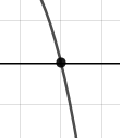
\includegraphics[width = 0.3\textwidth]{../Figures/polyZeroBehaviorAC.png}\item 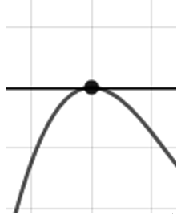
\includegraphics[width = 0.3\textwidth]{../Figures/polyZeroBehaviorBC.png}\item 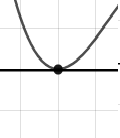
\includegraphics[width = 0.3\textwidth]{../Figures/polyZeroBehaviorCC.png}\item 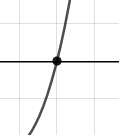
\includegraphics[width = 0.3\textwidth]{../Figures/polyZeroBehaviorDC.png}\end{multicols}\item None of the above.
\end{enumerate} }
\litem{
Which of the following equations \textit{could} be of the graph presented below?
\begin{center}
    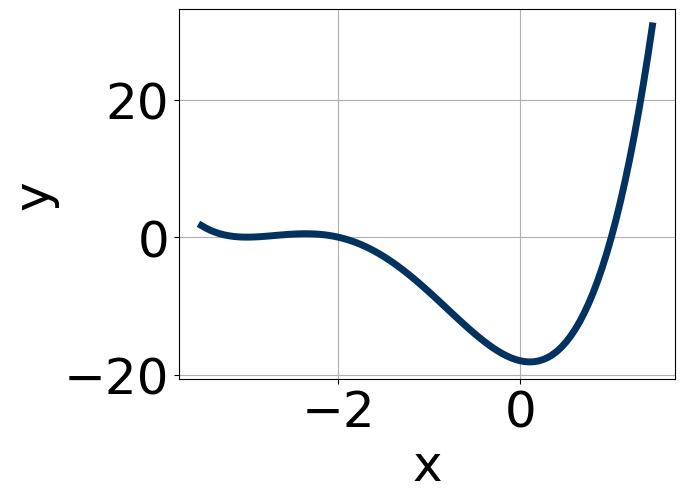
\includegraphics[width=0.5\textwidth]{../Figures/polyGraphToFunctionCopyC.png}
\end{center}
\begin{enumerate}[label=\Alph*.]
\item \( 17(x + 3)^{9} (x + 2)^{4} (x - 1)^{9} \)
\item \( 8(x + 3)^{4} (x + 2)^{5} (x - 1)^{9} \)
\item \( 11(x + 3)^{10} (x + 2)^{10} (x - 1)^{7} \)
\item \( -3(x + 3)^{8} (x + 2)^{5} (x - 1)^{9} \)
\item \( -3(x + 3)^{4} (x + 2)^{9} (x - 1)^{8} \)

\end{enumerate} }
\litem{
Describe the zero behavior of the zero $x = 6$ of the polynomial below.\[ f(x) = 5(x + 3)^{8}(x - 3)^{4}(x - 6)^{13}(x + 6)^{8} \]\begin{enumerate}[label=\Alph*.]
\begin{multicols}{2}\item 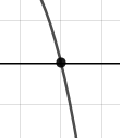
\includegraphics[width = 0.3\textwidth]{../Figures/polyZeroBehaviorCopyAC.png}\item 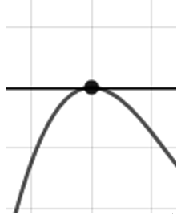
\includegraphics[width = 0.3\textwidth]{../Figures/polyZeroBehaviorCopyBC.png}\item 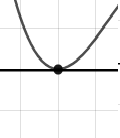
\includegraphics[width = 0.3\textwidth]{../Figures/polyZeroBehaviorCopyCC.png}\item 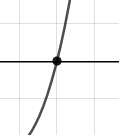
\includegraphics[width = 0.3\textwidth]{../Figures/polyZeroBehaviorCopyDC.png}\end{multicols}\item None of the above.
\end{enumerate} }
\litem{
Which of the following equations \textit{could} be of the graph presented below?
\begin{center}
    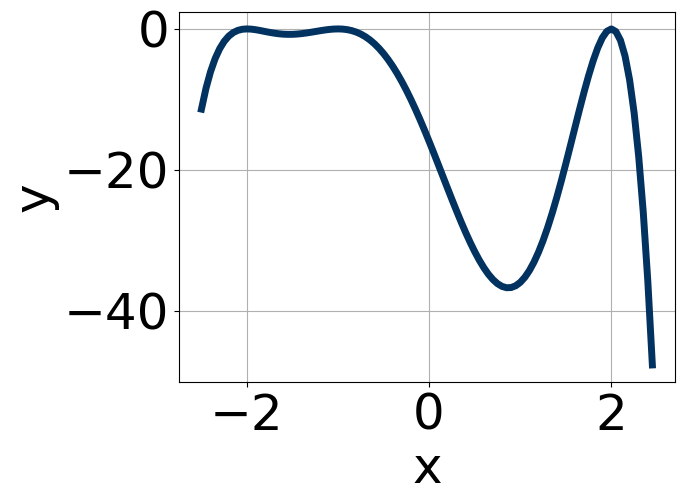
\includegraphics[width=0.5\textwidth]{../Figures/polyGraphToFunctionC.png}
\end{center}
\begin{enumerate}[label=\Alph*.]
\item \( 7(x - 2)^{4} (x + 2)^{6} (x + 1)^{9} \)
\item \( -4(x - 2)^{8} (x + 2)^{11} (x + 1)^{9} \)
\item \( 13(x - 2)^{4} (x + 2)^{8} (x + 1)^{6} \)
\item \( -19(x - 2)^{8} (x + 2)^{4} (x + 1)^{4} \)
\item \( -16(x - 2)^{6} (x + 2)^{4} (x + 1)^{11} \)

\end{enumerate} }
\litem{
Describe the end behavior of the polynomial below.\[ f(x) = 4(x + 5)^{5}(x - 5)^{10}(x - 2)^{3}(x + 2)^{5} \]\begin{enumerate}[label=\Alph*.]
\begin{multicols}{2}\item 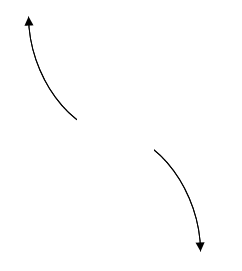
\includegraphics[width = 0.3\textwidth]{../Figures/polyEndBehaviorCopyAC.png}\item 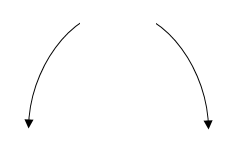
\includegraphics[width = 0.3\textwidth]{../Figures/polyEndBehaviorCopyBC.png}\item 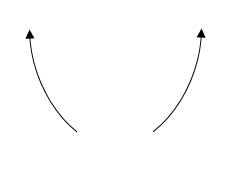
\includegraphics[width = 0.3\textwidth]{../Figures/polyEndBehaviorCopyCC.png}\item 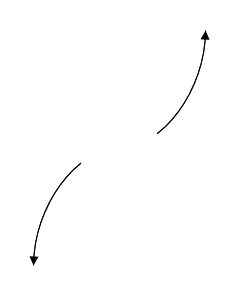
\includegraphics[width = 0.3\textwidth]{../Figures/polyEndBehaviorCopyDC.png}\end{multicols}\item None of the above.
\end{enumerate} }
\litem{
Describe the end behavior of the polynomial below.\[ f(x) = 4(x + 6)^{2}(x - 6)^{5}(x + 4)^{2}(x - 4)^{2} \]\begin{enumerate}[label=\Alph*.]
\begin{multicols}{2}\item 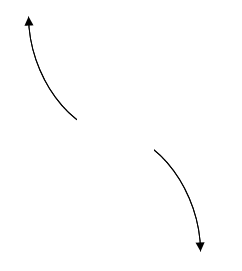
\includegraphics[width = 0.3\textwidth]{../Figures/polyEndBehaviorAC.png}\item 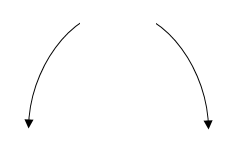
\includegraphics[width = 0.3\textwidth]{../Figures/polyEndBehaviorBC.png}\item 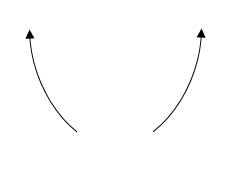
\includegraphics[width = 0.3\textwidth]{../Figures/polyEndBehaviorCC.png}\item 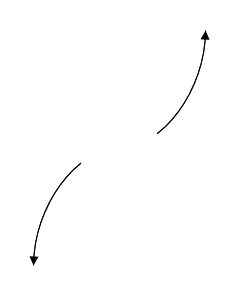
\includegraphics[width = 0.3\textwidth]{../Figures/polyEndBehaviorDC.png}\end{multicols}\item None of the above.
\end{enumerate} }
\end{enumerate}

\end{document}